\documentclass[12pt, twoside]{article}
\usepackage{jmlda}
\usepackage{bm}
\usepackage{amsmath}
\newcommand{\hdir}{.}

\begin{document}
\English

\title
	[] % short title for page headings, not necessary if a full title fits the headings
    {Additively Regularized Multimodal Topic Hierarchies} % full title
\author
	[] % short list of the authors (<= 3) for page headings, is necessary only if the full list does not fit the headings
	{N.\,A.~Chirkova, K.\,V.~Vorontsov} % full list of the authors, presented in the table of contetns of the issue
    [N.\,A.~Chirkova$^1$, K.\,V.~Vorontsov$^2$] % list of the authors presented in the title page of the article, is necessary only if it differs from the full list of the authors in braces, i.e. '{' and '}'
\email
    {nadiinchi@gmail.com, vokov@forecsys.ru}
\thanks
    {}
\organization
    {$^1$Lomonosov Moscow State University, Leninskie Gory, 1, Moscow, Russia;
     $^2$ORGANIZATION}
\abstract
    {AAA ``Machine Learning and Data Analysis''.
		
	\noindent
	BBB


	
	\noindent
	\textbf{Background}:	One paragraph about the problem, existent approaches and its limitations.
	
	\noindent
	\textbf{Methods}: One paragraph about proposed method and its novelty.
	
	\noindent
	\textbf{Results}: One paragraph about major properties of the proposed method and experiment results if applicable.
	
	\noindent
	\textbf{Concluding Remarks}: One paragraph about the place of the proposed method among existent approaches.
		
	\noindent
    	\textbf{Keywords}: \emph{topic modeling; ARTM; topic hierarchies; regularization}}

\titleRus
    [] % short title for page headings, not necessary if a full title fits the headings
    {Аддитивно регуляризованные многомодальные тематические иерархии} % full title
\authorRus
    [] % short list of the authors (<= 3) for page headings, is necessary only if the full list does not fit the headings
    {Н.\,А.~Чиркова, К.\,В.~Воронцов} % full list of the authors, presented in the table of contetns of the issue
    [Н.\,А.~Чиркова$^1$, К.\,В.~Воронцов$^2$] % list of the authors presented in the title page of the article, is necessary only if it differs from the full list of the authors in braces, i.e. '{' and '}'
\thanksRus
    {}
\organizationRus
    {$^1$Московский государственный университет им. М.\,В.\,Ломоносова $^2$Организация}
\abstractRus
    {
	
\bigskip
\noindent
\textbf{Ключевые слова}: \emph {тематическое моделирование; АРТМ;  тематические иерархии; регуляризация}
}


%these fields are filled in by the journal editors
\doi{10.21469/22233792}
\receivedRus{12.05.2016}
\receivedEng{May 12, 2016}

\maketitle
\linenumbers

\newcommand{\norm}{\mathop{\text{norm}}}

\section{Introduction}
\noindent %this command is placed at the beginning of the first sentence of each paragraph/section only.
Topic modeling is a popular technique for semantic analysis of text collections. Topic model defines each topic by a~probability distribution over words and describes each document by a~probability distribution over topics. 
In large text collections such as digital libraries or social media archives topics are usually organized in a hierarchy. Topic hierarchy helps user to navigate through collection: going down the hierarchy, user chooses interesting subtopics and finds a small subset of documents to read. Also hierarchy can help to detect the number of topics in collection if they will be modeled from major to specific.

A lot of research about automatic topic hierarchy learning was done in last years. There are different definitions of topic hierarchy in literature depending on main properties authors determine for their approach. Despite all this work there is still no common quality measure of topic hierarchies. It makes difficult to compare and tune hierarchical models.  

The basic drawback of all existing approaches to hierarchy learning is the difficulty of combining them with other modifications of topic models. These modifications include learning time- and location-specific topics, using additional information about texts in model, integrating topic models with other machine learning problems such as recommendations and classification. On the other hand, there is a novel approach that allows to blend different modifications in one topic model called Additive Regularization of Topic Models~\cite{ARTM}. This framework provides tools for handling multisource, or multimodal data, 
% Много ссылок на комбинации регуляризаторов в BigARTM.
it is well scalable for large collections~\cite{BigARTM} and is implemented in rich open-source topic modeling library BigARTM.

The goal of this work is to propose a method of learning topic hierarchies via topic model regularization and integrate it with ARTM. 

We focus on hierarchies as a multilevel graph of topics rather than a topic tree. While the last definition is a mainstream in literature, an assumption that a topic can inherit from several major topics looks more reasonable. 
It is common case in any field of knowledge when specific topic occurs on the edge of two or even more major topics. For example, bioinformatics combines applied mathematics and computer science to solve biology problems. This situation is called multiple inheritance.
Even if some approach supports multiple inheritance, almost none of them propose a method of sparsing topic graph so that a topic may have more than one but only few parent topics. Regularization allows us to meet this requirement too.
Finally, our approach automatically determines the number os subtopics for each topic.

Hence, we propose a scalable method of learning multimodal topic hierarchies with multiple inheritance that can be easily adapted to any specific task using regularization. The reminder of paper is organized as follows. In section~1 we overview existing approaches for learning hierarchies. In section~2 we give formal problem statement, then describe out approach in section~3 and its implementation in BigARTM in section~4. The last two sections are about experiments and discussion.

\section{Related Work}
\label{RelatedWork}
Two basic statistical topic modeling techniques are probabilistic latent semantic analysis (PLSA) and its Bayesian extension latent Dirichlet allocation (LDA). These are generative probabilistic models of word occurrence in a document. A lot of LDA expansions were developed to meet applications tasks: in~\cite{FindingBurstyTopics} generative model was improved to find topics that have bursty patterns on microblogs, in~\cite{CTR} topic model was merged with collaborative filtering probabilistic model to provide recommendations of previously unseen items. 

Additive Regularization of Topic Models~\cite{ARTM} is PLSA extension that allows to impose additional, subject-specific criteria for topic model parameters. Many of LDA expansions can be interpreted as regularization criteria, then different modifications will be combined in single model.
%%% ARTM citation?

These are flat models where all topics are treat as equal. In hierarchy topics are linked by parent-child relations.
Topic hierarchies are usually built in two ways: via generative model complication or as a combination of several ties flat models. Hierarchical Latent Dirichlet allocation~(hLDA)~\cite{hLDA} and hierarchical Pachinko Allocation Model~(PAM)~\cite{hPAM} are examples of first group. As other LDA extensions these models are trained using time consuming Gibbs Sampling that limits available collection size~\cite{STROD} and integration with other topic models modifications. hLDA is a tree structure and hPAM is a directed acyclic multilevel graph with no tools for edges number reduction.
% hLDA is a tree structure where each document passes a single path; hPAM is a directed acyclic multilevel graph where a document is assigned distributions over suptopics of each topic.

Second group approaches are split into top-down, constructing hierarchy from major topics to specialized, and bottom-up. Tree structured hierarchies are often learned top-down recursively: first a flat model with few topics is learned, then process repeats for each sub-topic. SplitLDA~\cite{splitLDA} splits documents between topics accordingly to distribution over topics for each document-word pair. Constructing A Topical
HierarchY~(CATHY) approach~\cite{CATHY} operates with phrases rather than words and divides them between subtopics. In Scalable and Robust Construction of Topic Hierarchies~(STROD)~\cite{STROD} each topic distribution over words can be expanded to a mixture of suptopics distributions using tensor decomposition algorithm. The drawback of recursive approaches is that they need heuristics to determine the number of subtopics in each topic. On the other hand, recursive learning is usually fast, STROD is proven~\cite{STROD} to be the fastest of all described approaches on large collections.

Multiple inheritance supporting hierarchies are usually learned level by level. In~\cite{Srivastava} hierarchy is learned in two steps: first, flat LDA models are learned for each level; next, topics between levels are linked using special subsumption criteria. An advantage is that changing threshold on subsumption criteria one can tune hierarchy sparsity. The disadvantage is that specific topics are modeled independently from their major topics. Also a simple agglomerative clustering based method for determining the number of topics in levels is proposed in this work. 

In~\cite{Zavitsanos} hierarchy is constructed bottom up. A great number of last level topics is learned first, then these topics are treat as pseudodocuments and next level model is learned from them. In this case subtopic-pseudodocument proportions specify topic graph structure and there is no ability to reduct edges count. Author emphasizes that the evaluation of topic hierarchies is an open issue.

Almost all hierarchical topic models are based on LDA, it makes difficult integrating other topic model modifications into hierarchy. We propose 
a top down hierarchy learning framework based on ARTM that incorporates few reasonable ideas from other approaches.

\section{Problem statement}
\label{ProblemStatement}
In this paper we refer to the document collection as $D$ consisting of documents of different subjects.
Documents may contain not only words but other elements too, say tags, links, location marks etc. We refer to such types of elements as modalities. For example, scientific paper can be described at least by three modalities: text, keywords and references. $M$ denotes a set of all modalities in the collection. Modalities $m \in M$ are defined by disjoint dictionaries $W = \bigsqcup_{m \in M} W^m$. 

A document $d \in D$ is a sequence of $n_d$ elements: $(w_1, w_2, w_3, \dots)$, $w_i \in W$. In this paper an order of elements is not important. Thus collection can be represented as a counters matrix $\{n_{dw}\}_{D \times W}$, $n_{dw}$ is a number of $w$ occurencies in $d$.

Given the text collection, our goal is to organize its documents into comprehensive hierarchical structure. We define \emph{topic hierarchy} as an oriented multipartitle (multilevel) graph of topics so that edges connect topics from neighboring levels. If there is an edge $a \rightarrow t$ in hierarchy then topic $a$ is called \emph{parent}, or \emph{ancestor} topic and $t$ is called \emph{child topic}, or \emph{subtopic}. Parent topic is divided into several more specific child topics. 
Obviously, number of topics on each following (child) level must be greater than on previous (parent) level. Zero level consists of only one topic called \emph{root}. An example of topic hierarchy is given on pic.~\ref{fg:hierarchy}.

Each topic in hierarchy is associated with distributions over each modality dictionary. This allows us to represent a topic by a top of most probable words saying what this topic is about. The same can be done with other modalities.
\begin{figure}[!th]
	\begin{center}
		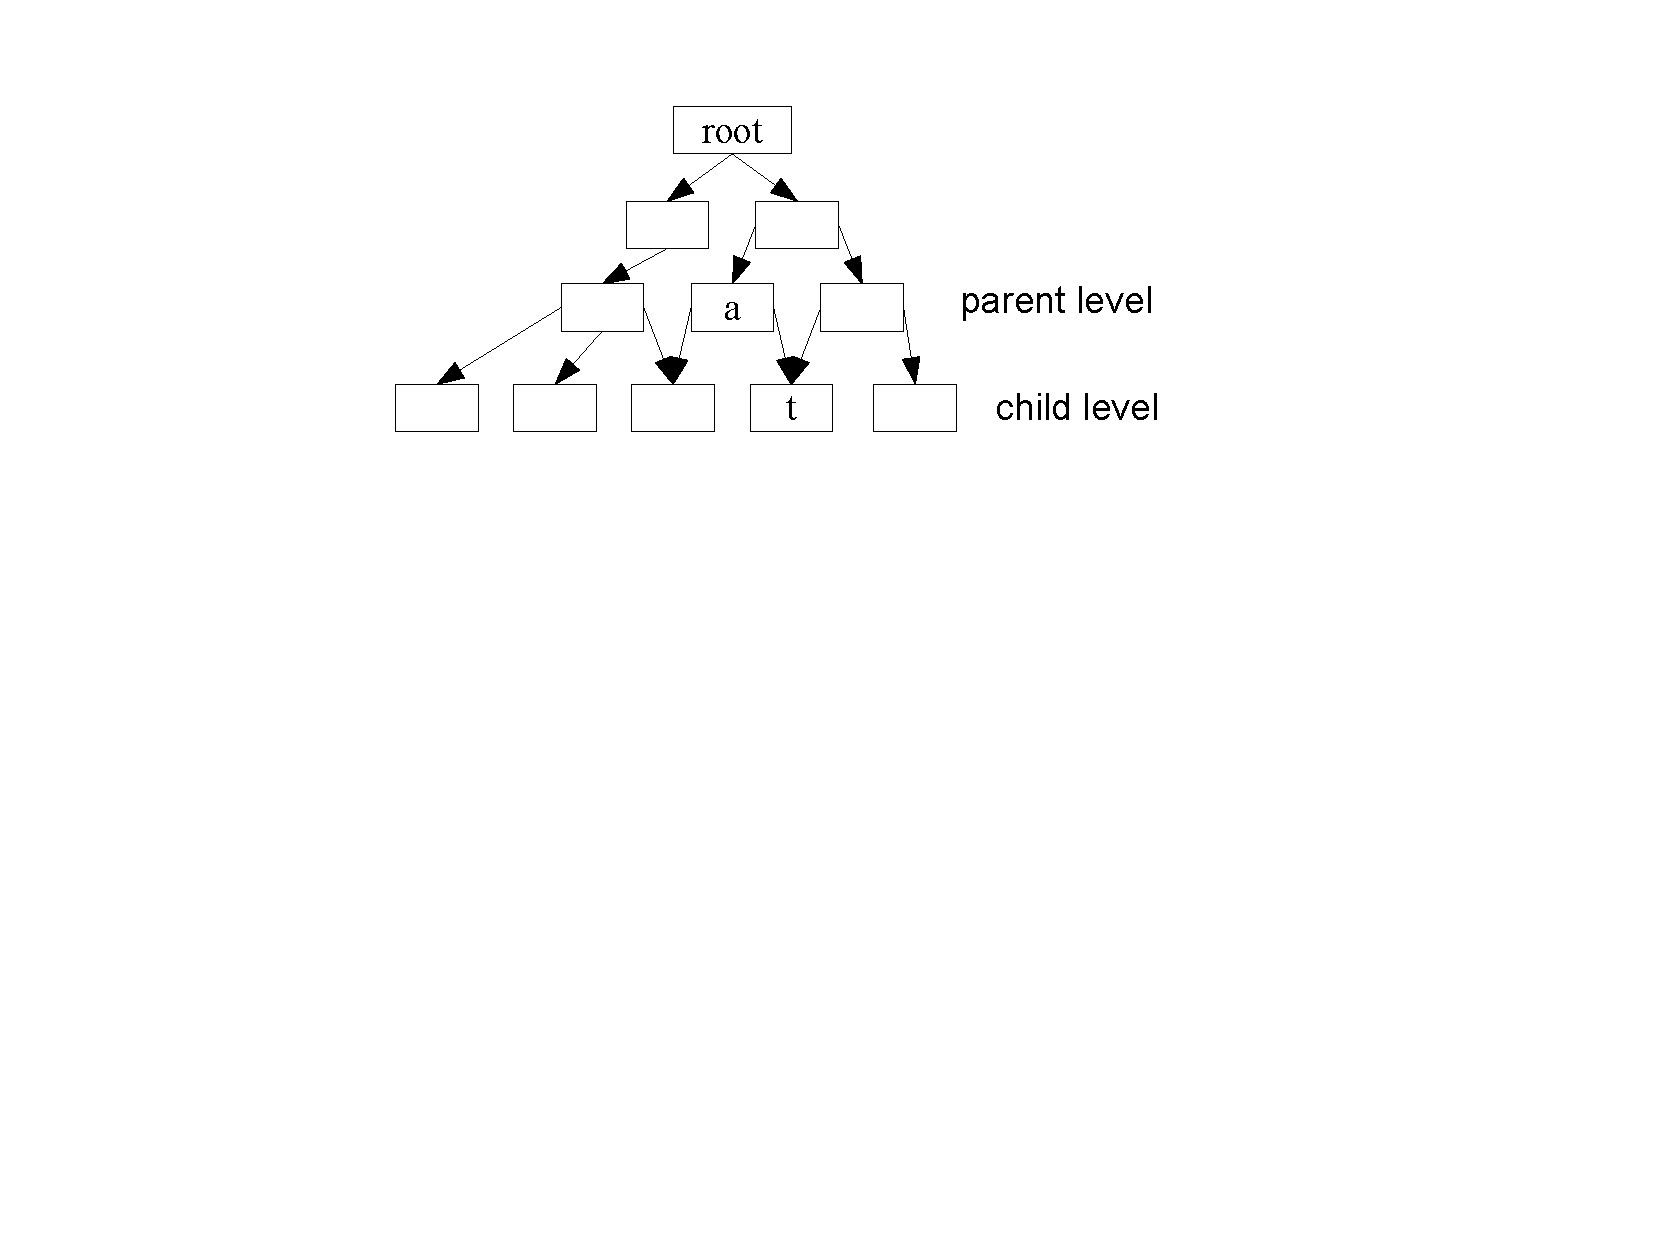
\includegraphics[width=0.4\linewidth]{\hdir/fig/hierarchy_definition.pdf}
	\end{center}
	\caption{An example of topic hierarchy}
	\label{fg:hierarchy}
\end{figure}

To learn hierarchy we learn several flat topic models and tie them via regularization.

In the rest of the paper we will use operator 
$\norm\limits_{x \in X} [y_x] = \frac{( y_x )_+}
{\sum_{x' \in X}( y_{x'})_+}$ transforming real vector to probability distribution, $(y_x)_+$ equals $y_x$ if $y_x > 0$ and $0$ otherwise.


%In such formulation each topic except root may have more than one parent topics. 

\section{hARTM framework}
\label{hARTM} 
\subsection{ARTM: flat topic models}
Plate topic model describes collection $D$ by finite topics set $T$. In ARTM~\cite{ARTM} document distribution over each modality is modeled as a mixture of topics distributions:
\[
p(w|d) \approx \sum_{t \in T} p(w|t) p(t|d)   \quad  d \in D, \, w \in W^m.
\]
In other words, for each modality $m$ topic model is a low-rank approximation 
\[
F^m\approx \Phi^m \Theta
\]
of frequency matrix $F^m = \{f_{wd}\}_{W^m \times D}$, $f_{wd} = \norm\limits_{w \in W^m} [n_{dw}]$ estimating $p(w|d)$ with parameters $\Phi^m = \{\phi_{wt}\}_{W^m \times T}$, $\phi_{wt} = p(w|t)$ and $\Theta = \{\theta_{td}\}_{T \times D}$, $\theta_{td} = p(t|d)$. $\Phi$ and $\Theta$ are stochastic matrices:
\begin{equation}
	\label{constrains}
\sum_{w \in W^m} \phi_{wt} = 1, \quad \sum_{t \in T} \theta_{td} = 1.
\end{equation}
For brevity we denote vertically stacked $\Phi^m$, $m \in M$ and $F^m$, $m \in M$ by $\Phi$ and $F$ respectively. Then topic model in approximate matrix factorization $F \approx \Phi \Theta$.
% Parameters $\Theta$ specify the proportions of topics in documents, or weights of topics in the mixture.

We use regularized weighted maximum log-likelihood principle to learn $\Phi$ and $\Theta$ :
\begin{equation}
\label{optimization_problem}
    \sum_{m \in M} \kappa_m \sum_{d \in D} \sum_{w \in W^m} n_{dw} \ln \sum_{t \in T} \phi_{wt} \theta_{td} + \sum_i \tau_i R_i(\Phi, \Theta) \rightarrow \max_{\Phi, \Theta}.
\end{equation}
Weights $\kappa_m$ are used to balance log-likehood of modalities. Regularizers $R_i$ impose additional subject-specific criteria for model parameters. Regularizer coefficients $\tau_i$ balance optimization of regularizers and log-likehood. If regularizer term $R = \sum_i \tau_i R_i(\Phi, \Theta)$ equals zero and there is only text modality then described model simplifies to PLSA.

\begin{Theorem}[Vorontsov, Potapenko, 2014]
If all regularizers are continuously differentiable on $\Phi$ and $\Theta$, then the stationary point of problem \eqref{optimization_problem} with constrains \eqref{constrains} satisfies the following system yielding EM-algorithm for model training:

\begin{equation}
\label{EM_alrorithm}
	\begin{split}
	 \text{E-step}: \quad & p(t|d, w) = \norm\limits_{t \in T} [\phi_{wt} \theta_{td}], \quad w \in W, \, d \in D ;\\
	 \text{M-step}: \quad & \phi_{wt} = \norm\limits_{w \in W^m} \biggl[n_{wt} + \frac{\partial R}{\partial \phi_{wt}} \phi_{wt}\biggr], \quad n_{wt} = \sum_{d \in D} n_{dw} p(t| d, w), \quad w \in W^m, t \in T, m \in M;\\
	 & \theta_{td} = \norm\limits_{t \in T} \biggl[n_{td} + \frac{\partial R}{\partial \theta_{td}} \theta_{td}\biggr], \quad n_{td} = \sum_{w \in W} n_{dw} p(t| d, w), \quad t \in T, d \in D.
	 \end{split}
\end{equation}
\end{Theorem}
EM-algorithm is obtained by applying the fixed point iteration method to the system. An initial guess is random.

\textbf{Sparsing regularizers.} Frequently used sparsing regularizer~\cite{ARTM} causes distributions $p(w|t)$ and $p(t|d)$ to be sparse meaning the majority of distribution's domain elements have zero probability. To achieve it Kullback–Leibler divergence between specified distribution $\bm \alpha$, usually uniform, and target distribution is maximized. For instance, $\Theta$-sparsing regularizer:
\[
\sum_{d \in D} KL(\bm \alpha \| \bm \theta_d) \rightarrow \max_{\Theta} 
\quad
\Leftrightarrow
\quad
R_1(\Theta) = 
 - \sum_{d \in D} \sum_{t \in T} \alpha_t \ln \theta_{td} \rightarrow \max_{\Theta},
\]
$\bm \theta_d$ denotes $\Theta$ column, for uniform distribution $\alpha_t = \frac 1 {|T|}$. Similarly for $\Phi^m$ sparsing with uniform specified distribution:
\[
R_2(\Phi^m) = -\sum_{t \in T} \sum_{w \in W^m} \frac 1 {|W^m|} \ln \phi^m_{wt} \rightarrow \max_{\Phi^m} \quad \forall m.
\] 
Modified M-step formulas for parameters update:
\begin{equation}
\label{sparsing_M_step}
\phi_{wt} = \norm\limits_{w \in W^m} \biggl[n_{wt} - \frac {\tau_1} {|W^m|}\biggr],
\quad
\theta_{td} = \norm\limits_{t \in T} \biggl[n_{td} - \frac {\tau_2} {|T|}\biggr].
\end{equation}

\vspace{0.5cm}
Hyperparameters of flat topic model are number of topics $|T|$, weights $\{\kappa_m\}_{m \in M}$ and regularization coefficients $\{\tau_i\}_{i}$. While learning topic hierarchy, we will need to train flat topic model for each level of hierarchy, every time with new hyperparameters settings.

\subsection{hARTM: top-down hierarchy learning}
Since topic hierarchy is a multilevel graph, we consider each level as a flat topic model. We propose top-down, level by level hierarchy learning algorithm. Zero level is associated with the whole collection. The first level contains small number of major topics. Starting from second level, we need not only to model topics, but also to establish parent-child topic relations. To do this, we introduce two additional matrix factorization problems and propose two new interchangeable regularizers based on them. 

Assume we have already learned $\ell \geqslant 1$ hierarchy levels. Now we will learn $(\ell+1)$-th level that is child level for $\ell$-th ancestor level. Not to confuse levels we denote parent level topics $a \in A$ and parameters $\Phi^\ell$, $\Theta^\ell$ instead of $t \in T$, $\Phi$ and $\Theta$ used for child level. Note that $\Phi^\ell$ and $\Theta^\ell$ are already modeled.

\textbf{$\Phi$ interlevel regularizer.}
We suppose that parent topic distribution over words and other modalities should be a mixture of child topics distributions:
\[
p(w|a) = \sum_{t \in T} p(w|t) p(t|a), \quad w \in W^m, \, a \in A.
\] 
% Гипотеза условной независимости?
This means an approximation 
\begin{equation}
\label{phi_approximation}
\Phi^\ell \approx \Phi \Psi
\end{equation}
 with new parameters matrix $\Psi = \{\psi_{ta}\}_{T \times A}$, $\psi_{ta} = p(t|a)$ containing \emph{interlevel distributions} of children topics in parent topic. If the measure of probability distributions dissimilarity is Kullback–Leibler divergence, we have the following regularizaion criteria:
\begin{equation}
\label{phi_regularizer}
\nonumber
 \sum_{a \in A} n_a \, KL(\bm \phi^{\ell, m}_a \| \Phi^m \, \bm \psi_a)  \rightarrow \min_{\Phi^m, \Psi}
\end{equation}
or, equivalently,
\[
R_3(\Phi^m, \Psi) = \sum_{a \in A} \sum_{w \in W^m} n_{wa} \ln \sum_{t \in T} \phi_{wt} \psi_{ta} \rightarrow \max_{\Phi^m, \Psi},
\]
$\bm \phi^{\ell, m}_a$ and $\bm \psi_a$ denote columns of $\Phi^{\ell, m}$ and $\Psi$ respectively. Weights $n_a = \sum_{w \in W^m} n_{wa}$ are imposed to balance parent topics proportionally to their size and to scale criteria up to log-likelihood scale, $n_{wa}$ are parent topic counters from EM-algorithm.
Regularizer criterias are weighted by modalities weights: 
\[
R_3(\Phi, \Psi) = \sum_{m \in M} \kappa_m R_3(\Phi^m, \Psi).
\]

This regularizer is equivalent to adding $|A|$ pseudodocuments to collection represented by $\{n_{wa}\}_{W \times A}$ columns. Then $\Psi$ forms additional columns to $\Theta$ corresponding to pseudodocuments.
Note than child level couldn't be trained only on pseudodocuments because internal dimension in approximation \eqref{phi_approximation} is higher than the minimum dimension of $\Phi^\ell$ and $\Phi$ will just copy columns of $\Phi^\ell$.

\textbf{$\Theta$ interlevel regularizer.}
The same idea may be applied for regularizing $\Theta$ instead of $\Phi$. Then for each document distribution over parent topics is a mixture of topic distributions:   % ???
\[
p(a|d) = \sum_{t \in T} p(a|t) p(t|d).
\]
Additional matrix approximation looks like
\begin{equation}
    \nonumber
    \Theta^\ell \approx \widetilde \Psi \Theta 
\end{equation}
with interlevel distributions $\widetilde \Psi = \{\tilde \psi_{at}\}_{A \times T}$, $\tilde \psi_{at} = p(a|t)$. This means that parent topic's documents set is a union of children's documents sets. Regularizer criteria:
\[
R_4(\Theta, \widetilde \Psi) = \sum_{a \in A} \sum_{d \in D} \theta^\ell_{ad} \ln \sum_{t \in T} \tilde \psi_{at} \theta_{td} \rightarrow \max_{\widetilde \Psi, \Theta}.
\]
To train child model with regularizer we add new modality $\tilde m$ corresponding to parent topics and consider document counters for this modality are $\theta^\ell_{ad}$. $\Theta$-regularizer coefficient will become modality weight and $\widetilde \Psi$ will correspond to $\Phi^{\tilde m}$.
\begin{figure}[!th]
	\begin{center}
	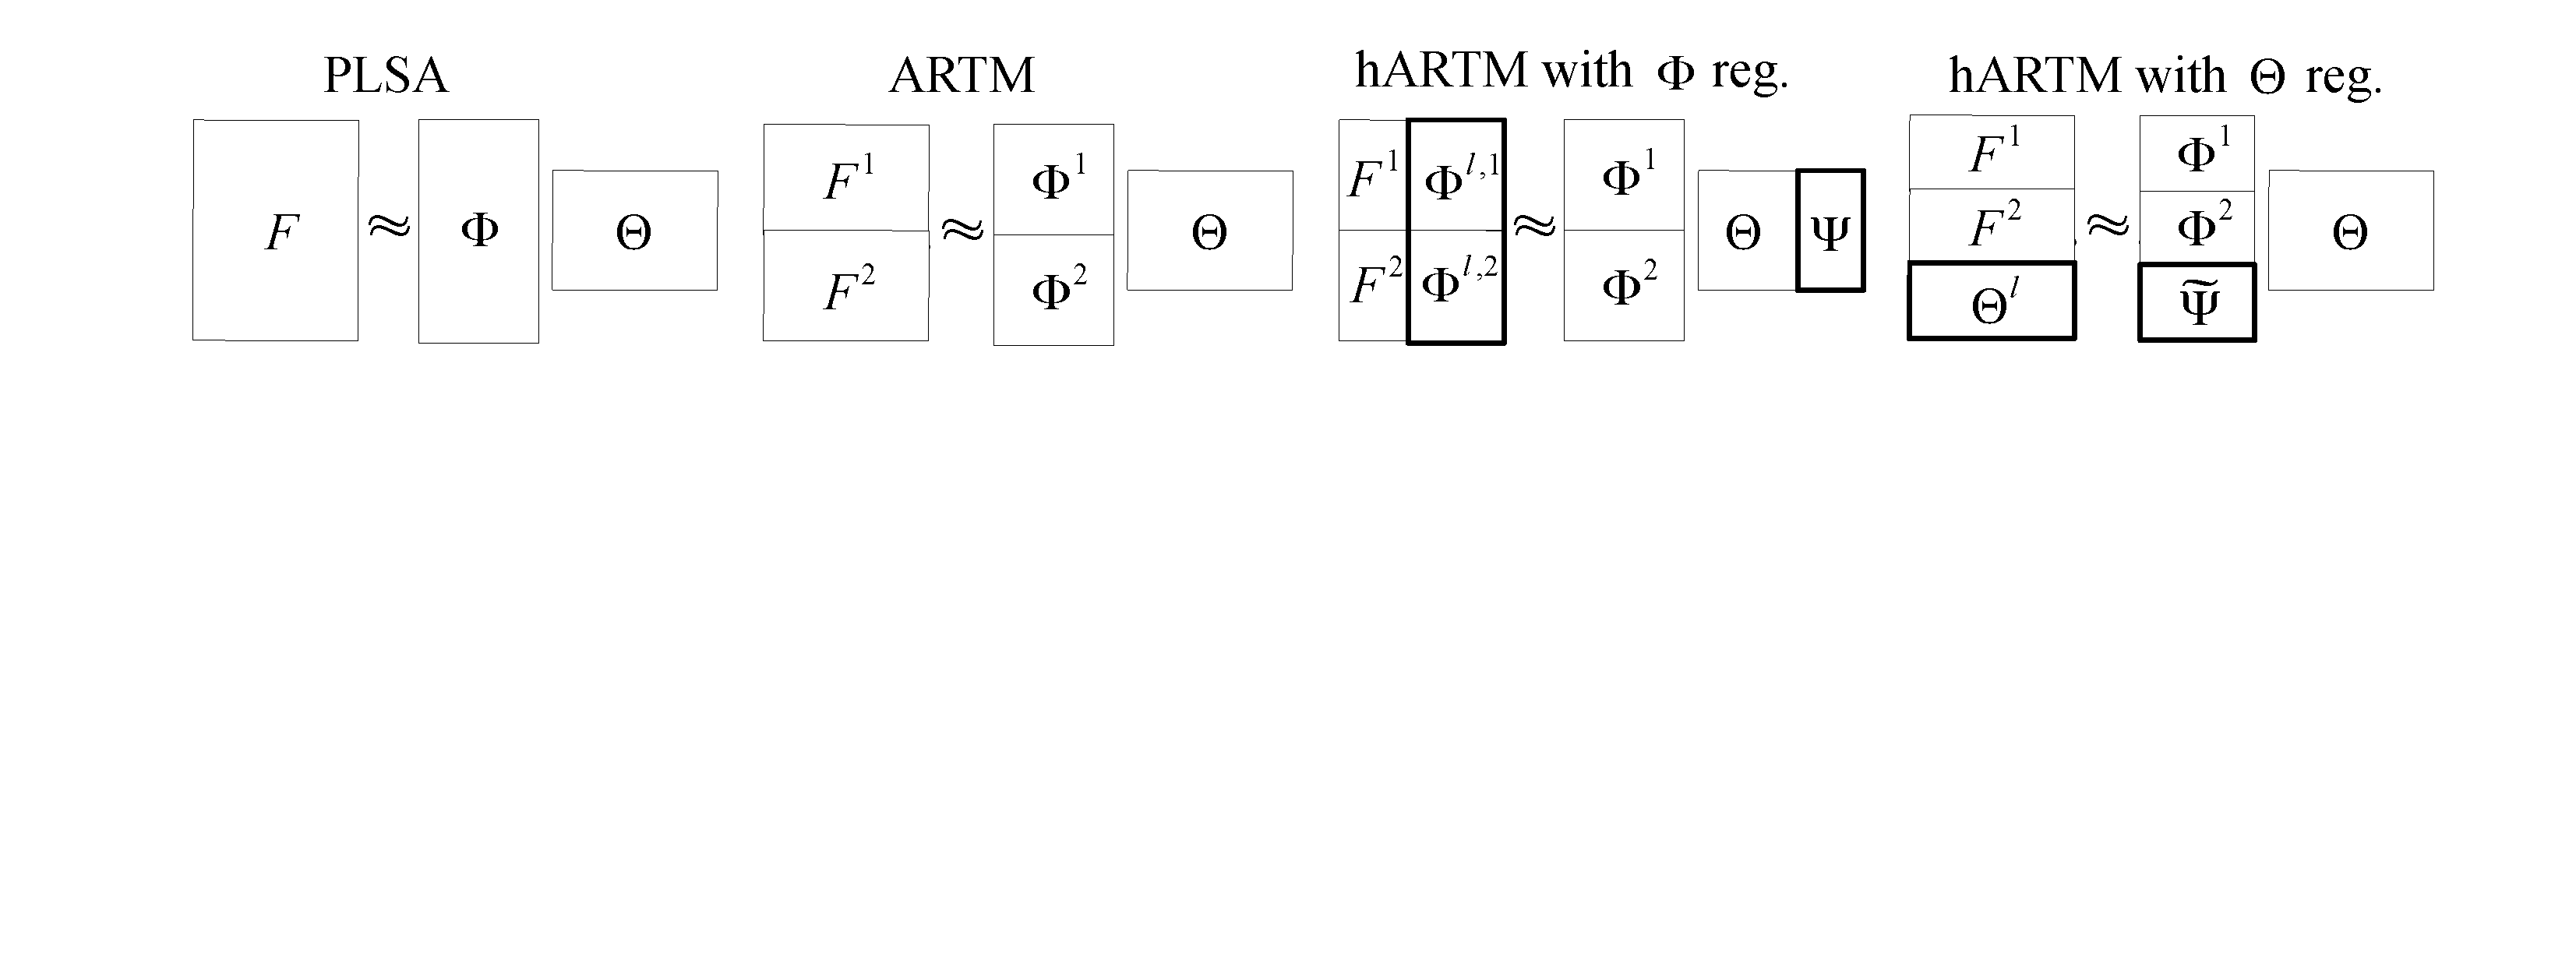
\includegraphics[width=\linewidth]{\hdir/fig/matrices_illustration_wide.pdf}
\end{center}
\caption{An illustration of child level regularization}
\label{fg:matrices}
\end{figure}

\vspace{0.5cm}
An illustration of manipulating with pseudodocuments and new modality while the regularization of child level is given on pic.~\ref{fg:matrices}.

\textbf{Hierarchy sparsing regularizers.}
When we allow topics to inherit from a number of parents we assume that this number won't be large, i.~e. 1--3, rarely greater parents. Such hierarchy is called \emph{sparse} one. In other words, we want distributions $p(a|t)$ to be sparse. Regularization allows us to achieve this requirement.

Since in $\Theta$ interlevel regularization approach $\widetilde \Psi$ is a child $\Phi^{\tilde m}$ and its columns represent distributions $p(a|t)$ we can use $\Phi$-sparsing regularizer described above to make the hierarchy sparse.
We rewrite \eqref{sparsing_M_step} replacing $\phi \rightarrow \tilde \psi$, $w \rightarrow a$, $W^m \rightarrow A$ to show how $\widetilde \Psi$ updates on each iteration:
\[
\tilde \psi_{at} = \norm\limits_{a \in A} \biggl[n_{at} - \frac {\tau_1} {|A|}\biggr].
\]

In case of $\Phi$ interlevel regularization $\Psi$ columns represent $p(t|a)$ distributions that can be converted to $p(a|t)$ using Bayes formula. Following the idea of other sparsing regularizers, we maximize KL-divergence between uniform distribution $\bm \gamma = \{\frac 1 {|A|}\}_{a \in A}$ and target one $\bm p_t = \{p(a|t)\}_{a \in A}$:
\[
\sum_{t \in T} KL(\bm \gamma \| \bm p_t) \rightarrow \max_{\Psi} 
\]
or, equivalently,
\[
R_5(\Psi) = \sum_{t \in T} \sum_{a \in A} \frac 1 {|A|} \ln p(a|t) = 
 \frac 1 {|A|} \sum_a \sum_t \ln \frac{\psi_{ta} \, p(a)} {\sum_{a'} \psi_{ta'} \, p(a')} \rightarrow \min_{\Psi}.
\]

To show how $\Psi$ updates we rewrite M-step formula in \eqref{EM_alrorithm} replacing $\theta \rightarrow \psi$ and $d \rightarrow a$ and taking derivatives of $R_5(\Psi)$ with respect to $\psi_{ta}$:
\[
\psi_{ta} = \norm\limits_{t \in T} \Biggl[n_{ta} - \tau_5 \biggl( \frac {1} {|A|} - p(a|t) \biggr)\Biggr].
\]
For each topic $t$ parent topics $a$ with high $p(a|t)$ get higher and parents with low $p(a|t)$ get lower. Note that $R_5$ cannot zeroize all components of $\Psi$ column whereas $R_1$ can do this with $\widetilde \Psi$ column.

\vspace{0.5cm}
\textbf{Hierarchy learning scenario.}
Thus, hyperparameters of topic hierarchy are number of levels, number of topics on each level, modalities weights and regularization coefficients.
One can learn hierarchy level by level, on each level finding parents for topics from previous level using $\Phi$ ot $\Theta$ interlevel rgularizer. If sparse hierarchy is desired, hierarchy sparsing regularizer should be also used. The process of training levels is stopped when topics on the last level are highly specialized. 

Regularization coefficients may be tuned for each level individually or used the same for all levels.
Note that when learning $(\ell+1)$-th level only $\ell$-th level's topics are used for regularization, not all previous levels' topics.

When hierarchy is learned, topics on each level are represented by its distributions over words and other modalities. Documents on each level are assigned to several topics with proportions specified in this level's $\Theta$ matrix. The hierarchy structure is defined by interlevel distributions. To draw the topic graph one may impose a threshold on $p(a|t)$ or $p(t|a)$.

\section{Implementation in BigARTM, open-source topic modeling library}
\label{BigARTM} 

\section{Experiments}

\section{Discussion}
%High rank, only as regularizer. Idea similar to Zavitsanos.

%%%% please specify doi of the cited item if possible, see~\bibitem{article}
%%%% Crossref doi of the item can be retrieved at http://www.crossref.org/guestquery/
\begin{thebibliography}{99}

\bibitem{book}
	\BibAuthor{Goossens,~M., F. Mittelbach, and A.~Samarin}. 1994.
	\BibTitle{The \LaTeX\ companion}.
	2nd ed.
	Reading, MA: Addison-Wesley. 528 p.

\bibitem{article}
	\BibAuthor{Zagurenko,~A.\,G., V.\,A.~Korotovskikh, A.\,A.~Kolesnikov, A.\,V.~Timonov, and D.\,V.~Kardymon}. 2008.
	Tekhniko-ekonomicheskaya optimizatsiya dizayna gidrorazryva plasta
	[Technical and economic optimization of the design of hydraulic fracturing].
	\BibJournal{Neftyanoe Khozyaystvo} [Oil Industry] 11(1):54--57.
	\BibDoi{10.3114/S187007708007}. (In Russian)

\bibitem{webArticle}
	\BibAuthor{Blaga,~P.\,A.} 2007.
	Commutative Diagrams with XY-pic II. Frames and Matrices.
	\BibJournal{PracTEX J.}  4.
	Available at: \BibUrl{https://tug.org/pracjourn/2007-1/blaga/blaga.pdf}
    (accessed February 20, 2007).

\bibitem{webResource}
	XYpic.
	Available at: \BibUrl{http://akagi.ms.u-tokyo.ac.jp/input9.pdf}
	(accessed April 09, 2015).

\bibitem{inproceedingsRus}
	\BibAuthor{Usmanov,~T.\,S., A.\,A.~Gusmanov, I.\,Z.~Mullagalin, R.\,Yu.~Mukhametshina, A.\,N.~Chervyakova, and A.\,V.~Sveshnikov.} 2007.
	Osobennosti proektirovaniya razrabotki mestorozhdeniy s primeneniem gidrorazryva plasta
	[Features of the design of field development with the use of hydraulic fracturing].
	\BibJournal{6th Symposium (International) ``New Energy Saving Subsoil Technologies and the
	Increasing of the Oil and Gas Impact'' Proceedings}.
	Moscow:~Publisher. 267--272. (In Russian)
	   	
\bibitem{inproceedingsEng}
    \BibAuthor{Author,~N.} 2009.
    Paper title.
    \BibJournal{10th Conference (International) on Any Science Proceedings}.
    Place of publication: Publisher. 111--122.
	
\bibitem{techreport}
	\BibAuthor{Lambert,~P.} 1993.
  	\BibTitle{The title of the work}.
  	Place of publication:~The institution that published.  Report~2.
  	     	
\end{thebibliography}

\maketitleSecondary
\Russian
%%%% please specify doi of the cited item if possible, see~\bibitem{article}
%%%% Crossref doi of the item can be retrieved at http://www.crossref.org/guestquery/
\begin{thebibliography}{99}
\bibitem{book}
    \BibAuthor{Гуссенс~М., Миттельбах~Ф., Cамарин~А.}
    \BibTitle{Путеводитель по пакету \LaTeX\ и~его расширению \LaTeXe} / Пер. с англ.~---
    М.:~Мир, 1999. 606~с.
    (\BibAuthor{Goossens M., Mittelbach F., Samarin A.}
     \BibTitle{The \LaTeX\ companion}.~--- 2nd ed.~--- Reading, MA, USA: Addison-Wesley, 1994. 528 p.)

\bibitem{article}
    \BibAuthor{Загуренко~А.\,Г., Коротовских~В.\,А., Колесников~А.\,А., Тимонов~А.\,В., Кардымов~Д.\,В.}
    Технико-экономическая оптимизация дизайна гидроразрыва пласта~//
    \BibJournal{Нефтяное хозяйство}, 2008. Т.~11. \No\,1. С.~54--57.
	\BibDoi{10.3114/S187007708007}.

\bibitem{webArticle}
	\BibAuthor{Blaga~P.\,A.}
	Commutative Diagrams with XY-pic II. Frames and Matrices~//
	\BibJournal{PracTEX J.}, 2007. Vol.\,4.
	URL: \BibUrl{https://tug.org/pracjourn/2007-1/blaga/blaga.pdf}.

\bibitem{webResource}
	XYpic.
	URL: \BibUrl{http://akagi.ms.u-tokyo.ac.jp/input9.pdf}.
	
\bibitem{inproceedingsRus}
	\BibAuthor{Усманов~Т.\,С., Гусманов~А.\,А., Муллагалин~И.\,З., Мухаметшина~Р.\,Ю., Червякова~А.\,Н., Свешников~А.\,В.}
	Особенности проектирования разработки месторождений с применением гидроразрыва пласта~//
	\BibJournal{Труды 6-го Междунар. симп. <<Новые ресурсосберегающие технологии недропользования и повышения нефтегазоотдачи>>}.~---
	М.:~Издательство, 2007. С.~267--272.

\bibitem{inproceedingsEng}
    \BibAuthor{Author~N.}
    Paper title~//
    \BibJournal{10th Conference (International) on Any Science Proceedings}.~---
    Place of publication: Publisher, 2009. P.~111--122.

\bibitem{techreport}
	\BibAuthor{Lambert~P.}
  	\BibTitle{The title of the work}.
  	Place of publication:~The institution that published, 1993.  Report~2.
 	
\end{thebibliography}


\end{document}
